% =========================================================
% 第二十八屆決策分析研討會 (DAS 2026) 論文 LaTeX 模板
% =========================================================
% 根據官方 Word 格式說明製作
% 編譯方式：XeLaTeX（支援中文）
%   xelatex DAS2026_template.tex
% =========================================================

\documentclass[12pt, a4paper]{article}

% ── 頁面設定（上下左右各 3 公分）─────────────────────────
\usepackage[
  a4paper,
  top=3cm, bottom=3cm,
  left=3cm, right=3cm
]{geometry}

% ── 字體（XeLaTeX）────────────────────────────────────────
\usepackage{fontspec}
\usepackage{xeCJK}

% 中文主字體：依環境自動回退，避免 fontspec 找不到字型而編譯失敗
\IfFontExistsTF{TW-Kai}{
  \setCJKmainfont[AutoFakeBold=true, AutoFakeSlant=true]{TW-Kai}
}{
  \IfFontExistsTF{BiauKai}{
    \setCJKmainfont[AutoFakeBold=true, AutoFakeSlant=true]{BiauKai}
  }{
    \IfFontExistsTF{PingFang TC}{
      \setCJKmainfont[AutoFakeBold=true, AutoFakeSlant=true]{PingFang TC}
    }{
      \setCJKmainfont[AutoFakeBold=true, AutoFakeSlant=true]{Noto Serif CJK TC}
    }
  }
}
\IfFontExistsTF{TW-MOE-Std-Kai}{
  \setCJKmonofont{TW-MOE-Std-Kai}
}{
  \IfFontExistsTF{Noto Serif CJK TC}{
    \setCJKmonofont{Noto Serif CJK TC}
  }{
    \setCJKmonofont{PingFang TC}
  }
}

% 英文 / 數字字體：Times New Roman（遵照格式規定）
\setmainfont{Times New Roman}

% ── 行距、段落────────────────────────────────────────────
\usepackage{setspace}
\singlespacing                       % 單行間距

\usepackage{indentfirst}
\setlength{\parindent}{2em}          % 首行縮排 2 個中文字元
\setlength{\parskip}{0pt}            % 段落間不留空白

% ── 標題、節次格式────────────────────────────────────────
\usepackage{titlesec}

% 一級標題：粗體 12pt，左對齊，上方留一行，下方留一行（空行）
\titleformat{\section}
  {\normalfont\bfseries\fontsize{12pt}{14pt}\selectfont}
  {\thesection.}{0.5em}{}
\titlespacing*{\section}{0pt}{12pt}{12pt}   % 上 12pt、下 12pt（約一行）

% 二級標題：粗體 12pt，左對齊
\titleformat{\subsection}
  {\normalfont\bfseries\fontsize{12pt}{14pt}\selectfont}
  {\thesubsection}{0.5em}{}
\titlespacing*{\subsection}{0pt}{12pt}{12pt}

% ── 圖、表、方程式────────────────────────────────────────
\usepackage{graphicx}
\usepackage{float}
\usepackage{caption}
\usepackage{subcaption}
\captionsetup[figure]{position=below,justification=centering,labelsep=space,font={small},singlelinecheck=true}
\captionsetup[table]{position=above,justification=centering,labelsep=space,font={small},singlelinecheck=true}
\renewcommand{\figurename}{圖}
\renewcommand{\tablename}{表}

\usepackage{amsmath}
\usepackage{amssymb}
\usepackage{booktabs}
\usepackage{array}
\usepackage{url}
\usepackage{hyperref}
\usepackage{natbib}
\bibliographystyle{apalike}

\newcommand{\eqbefore}{\vspace{0.5\baselineskip}}
\newcommand{\eqafter}{\vspace{0.5\baselineskip}}

% 圖標題：置於圖下方，置中
\captionsetup[figure]{
  position = below,
  justification = centering,
  labelsep = space,           % "圖1 " 格式
  font = {normalsize},
  singlelinecheck = true
}

% 表標題：置於表上方，置中
\captionsetup[table]{
  position = above,
  justification = centering,
  labelsep = space,
  font = {normalsize},
  singlelinecheck = true
}

% 中文圖表標籤
\renewcommand{\figurename}{圖}
\renewcommand{\tablename}{表}

% 方程式前後各空一行（\vspace 在正文中使用）

% ── 超連結────────────────────────────────────────────────

% ── 參考文獻────────────────────────────────────────────────
% 格式：作者年代法（Author-Year），中文在前，英文在後
% 如使用 BibTeX，可改用 natbib；此模板提供手動範例
\usepackage{natbib}
\bibliographystyle{apalike}   % APA 格式近似 DAS 引用規定

% ── 其他常用套件────────────────────────────────────────────
\usepackage{booktabs}         % 美觀表格線
\usepackage{array}
\usepackage{url}

% =========================================================
\begin{document}

\begin{center}\textit{第二十八屆決策分析研討會}\end{center}

\begin{center}
{\fontsize{14pt}{18pt}\selectfont\bfseries 太陽能板安裝地區潛力預測模型}
\end{center}
\vspace{4pt}

\begin{center}
林湘庭\textsuperscript{1}\quad 張佑丞\textsuperscript{2}\quad 藍柏婷\textsuperscript{3}\quad
李倢安\textsuperscript{4}\quad 柯絲昀\textsuperscript{5}

\vspace{2pt}
\textsuperscript{1--5}國立臺灣大學資訊管理學系\\[2pt]
\textsuperscript{1}\href{mailto:b12705008@ntu.edu.tw}{b12705008@ntu.edu.tw}\quad
\textsuperscript{2}\href{mailto:b12705055@ntu.edu.tw}{b12705055@ntu.edu.tw}\quad
\textsuperscript{3}\href{mailto:b12705030@ntu.edu.tw}{b12705030@ntu.edu.tw}\quad
\textsuperscript{4}\href{mailto:b12705041@ntu.edu.tw}{b12705041@ntu.edu.tw}\quad
\textsuperscript{5}\href{mailto:b12705066@ntu.edu.tw}{b12705066@ntu.edu.tw}
\end{center}
\vspace{8pt}

\noindent\textbf{摘要}

\noindent
太陽能部署受氣候、住宅條件、經濟承載力與政策誘因共同影響，但多數既有預測模型建立於單一國家情境，難以直接用於臺灣。
本研究以 Stanford DeepSolar 資料集為基礎，提出一套可跨國遷移的決策支持流程。
首先，系統篩除美國特有政策、族裔與地理識別欄位，保留可泛化特徵；
其次，以 Two-Stage 架構建立美國基準模型，區分「是否部署」與「部署強度」兩個子問題；
最後，整合臺灣鄉鎮級氣候、收入、人口與住宅資料，推論 368 個鄉鎮市區之太陽能潛力，並以 TOPSIS 排定推廣優先序。
為避免縣市層級常數誤導鄉鎮排序，本研究僅將真正具鄉鎮差異的指標納入 MADA，將 FIT、教育與就業視為縣市背景資訊。
結果顯示，Two-Stage 模型於美國測試集具良好表現（Stage~1 F1 = 0.894；Stage~2 $R^2=0.750$），而在臺灣的排序結果與實際太陽光電裝設量亦呈正相關；
以縣市平均鄉鎮潛力對每鄉鎮平均裝設量檢驗，Spearman $\rho=0.600$（$p=0.003$），若以縣市總分對縣市總裝設量檢驗，則達 $\rho=0.878$（$p<0.001$）。
研究結果顯示，跨國遷移式太陽能潛力建模可作為政府與業者進行區域推廣決策的實用工具。

\vspace{4pt}
\noindent\textbf{關鍵字：}太陽能部署預測、特徵選擇、機器學習、多屬性決策分析、跨國遷移推論

\vspace{8pt}

% =========================================================
\section{緒論}
% =========================================================

太陽能發電為全球能源轉型之關鍵技術，其部署普及受氣候條件、經濟承載力與政策誘因等多重因素影響。
準確識別高潛力地區，有助於太陽能業者安排市場開發順序，也能協助政府更精準配置推廣資源。
Stanford DeepSolar 以美國逾 73,000 個人口普查區建立太陽能部署預測模型，為此議題提供了具代表性的資料基礎 \citep{dubey2021deepsolar}；
但其特徵包含美國特有政策、族裔與地理識別欄位，無法直接移植到臺灣。

因此，本研究聚焦一個更實務的問題：若希望沿用 DeepSolar 的建模邏輯到臺灣，我們應如何保留可遷移訊號、移除不可遷移特徵，並將模型輸出轉化為可操作的推廣優先序？
本文的故事線依序為：
（1）建立可跨國泛化的特徵集合；
（2）訓練美國 Two-Stage 基準模型；
（3）整合臺灣鄉鎮級資料進行潛力推論；
（4）以僅含鄉鎮差異訊號的 TOPSIS 進行排序；
（5）以臺灣實際裝設量做外部驗證。

\subsection{研究貢獻}

相較於僅在單一國家情境中追求預測準確度之研究，本文更重視模型在跨國決策支持上的可用性。
本研究之主要貢獻可歸納為三點。
首先，在資料面上，本文提出一套可操作的特徵遷移原則，將原始 DeepSolar 中高度美國在地化的欄位系統性區分為「可保留」與「應排除」兩類，降低跨國應用時的任意性。
其次，在模型面上，本文保留 Two-Stage 架構，以部署與否及部署強度分而治之，兼顧分類辨識與迴歸解釋。
最後，在決策面上，本文不直接將所有可得指標混入排序，而是進一步區分鄉鎮層級訊號與縣市背景資訊，避免 MADA 因尺度或行政層級不一致而產生偏誤。
此一流程使模型結果不僅可用於預測，更可進一步支援區域推廣優先序之討論。

% =========================================================
\section{資料與特徵篩選}
% =========================================================

\subsection{資料來源}

本研究使用 Stanford DeepSolar 資料集 \citep{dubey2021deepsolar}，涵蓋美國 72,537 個人口普查區、169 個欄位，目標變數為 \texttt{tile\_count}（各地區現有太陽能板數量）。
欄位可概分為太陽能相關、電力經濟、氣候條件、社經統計、住宅特徵、政策激勵及地理識別碼等群組。

\subsection{不可遷移特徵篩除}

為建立可跨國泛化之特徵集合，本研究先排除三類欄位：
（1）美國特有政策與行政識別欄位；
（2）族裔與區域專屬人口結構欄位；
（3）與目標變數高度重疊之洩漏欄位。
篩除後保留 131 個候選特徵。
此處之核心考量並非單純降低維度，而是確保後續保留之變數在概念上仍具有跨國可比性。
例如氣候、電力消費、人口密度、家戶收入與住宅自有率等變數，雖然在不同國家之量尺與分布不盡相同，但其作為太陽能部署條件之經濟與行為意涵仍具一致性。

\subsection{特徵篩選流程}

本研究以三步驟降低共線性與維度：
先移除高度相關變數對（$|r|>0.85$）中的冗餘欄位，再綜合 Lasso、ElasticNet 與隨機森林三種嵌入式方法做投票，保留至少兩種方法選中之變數，形成 90 個特徵的 \textbf{Voted 特徵集}；
最後再以 VIF 檢查多重共線性，得到 55 個特徵的 VIF 特徵集。
後續 Two-Stage 模型以 Voted 特徵集為主。
採用投票式篩選而非單一方法的理由，在於不同方法對線性稀疏性與非線性重要性的敏感度不同。
透過保留多方法共同支持的特徵，可在泛化性與解釋性之間取得較穩健的平衡。

% =========================================================
\section{Two-Stage 預測模型}
% =========================================================

\subsection{模型架構}

本研究沿用原論文 SolarForest 的 Two-Stage 架構設計邏輯，將預測問題拆解為部署與否及部署強度兩個子問題：
\eqbefore
\begin{align}
\text{Stage 1: } & \hat{y}_1 = \mathbb{I}(\text{tile\_count} > 0) \quad \text{（部署與否二分類）} \\
\text{Stage 2: } & \hat{y}_2 = \log\bigl(1 + \tfrac{\text{tile\_count}}{\text{household\_count}} \times 1000\bigr) \quad \text{（已部署地區之每千戶密度迴歸）}
\end{align}
\eqafter

此拆解可避免零膨脹（zero-inflation）問題直接干擾迴歸學習。
Stage~1 使用 RandomForestClassifier（300 棵樹，\texttt{class\_weight='balanced'}），Stage~2 使用 RandomForestRegressor（200 棵樹），缺失值以中位數填補。
之所以採用樹模型而非單純線性模型，一方面是考量太陽能部署與社經條件之間可能存在非線性交互作用，另一方面則是隨機森林對缺失值填補後的混合型特徵具有較佳穩健性。

\subsection{模型評估結果}

表 \ref{tab:twostage_metrics} 彙整 Two-Stage 模型於保留測試集（20\%，分層採樣）之表現。
Stage~1 分類器之 F1 分數達 0.894、ROC-AUC 達 0.864，顯示模型能有效辨識已部署地區；
Stage~2 迴歸器之 $R^2$（log1p 尺度）達 0.750，MAE 為 0.547。

\begin{table}[H]
\caption{Two-Stage 模型保留測試集表現（Voted 特徵集，90 欄）}
\label{tab:twostage_metrics}
\centering
\small
\begin{tabular}{lcccc}
\toprule
Stage & 指標 & 數值 & 指標 & 數值 \\
\midrule
Stage 1（分類） & Accuracy & 0.825 & Precision & 0.844 \\
& F1-Score & 0.894 & Recall & 0.950 \\
& ROC-AUC & 0.864 & & \\
\midrule
Stage 2（迴歸） & $R^2$（log1p） & 0.750 & RMSE（log1p） & 0.731 \\
& MAE（log1p） & 0.547 & & \\
\bottomrule
\end{tabular}
\end{table}

圖 \ref{fig:twostage_results} 顯示 Stage~1 與 Stage~2 的核心表現。
整體而言，美國基準模型已具備足夠穩定的辨識能力，可作為後續臺灣遷移推論之基礎。

\begin{figure}[H]
\centering
\begin{minipage}[b]{0.45\linewidth}
\centering
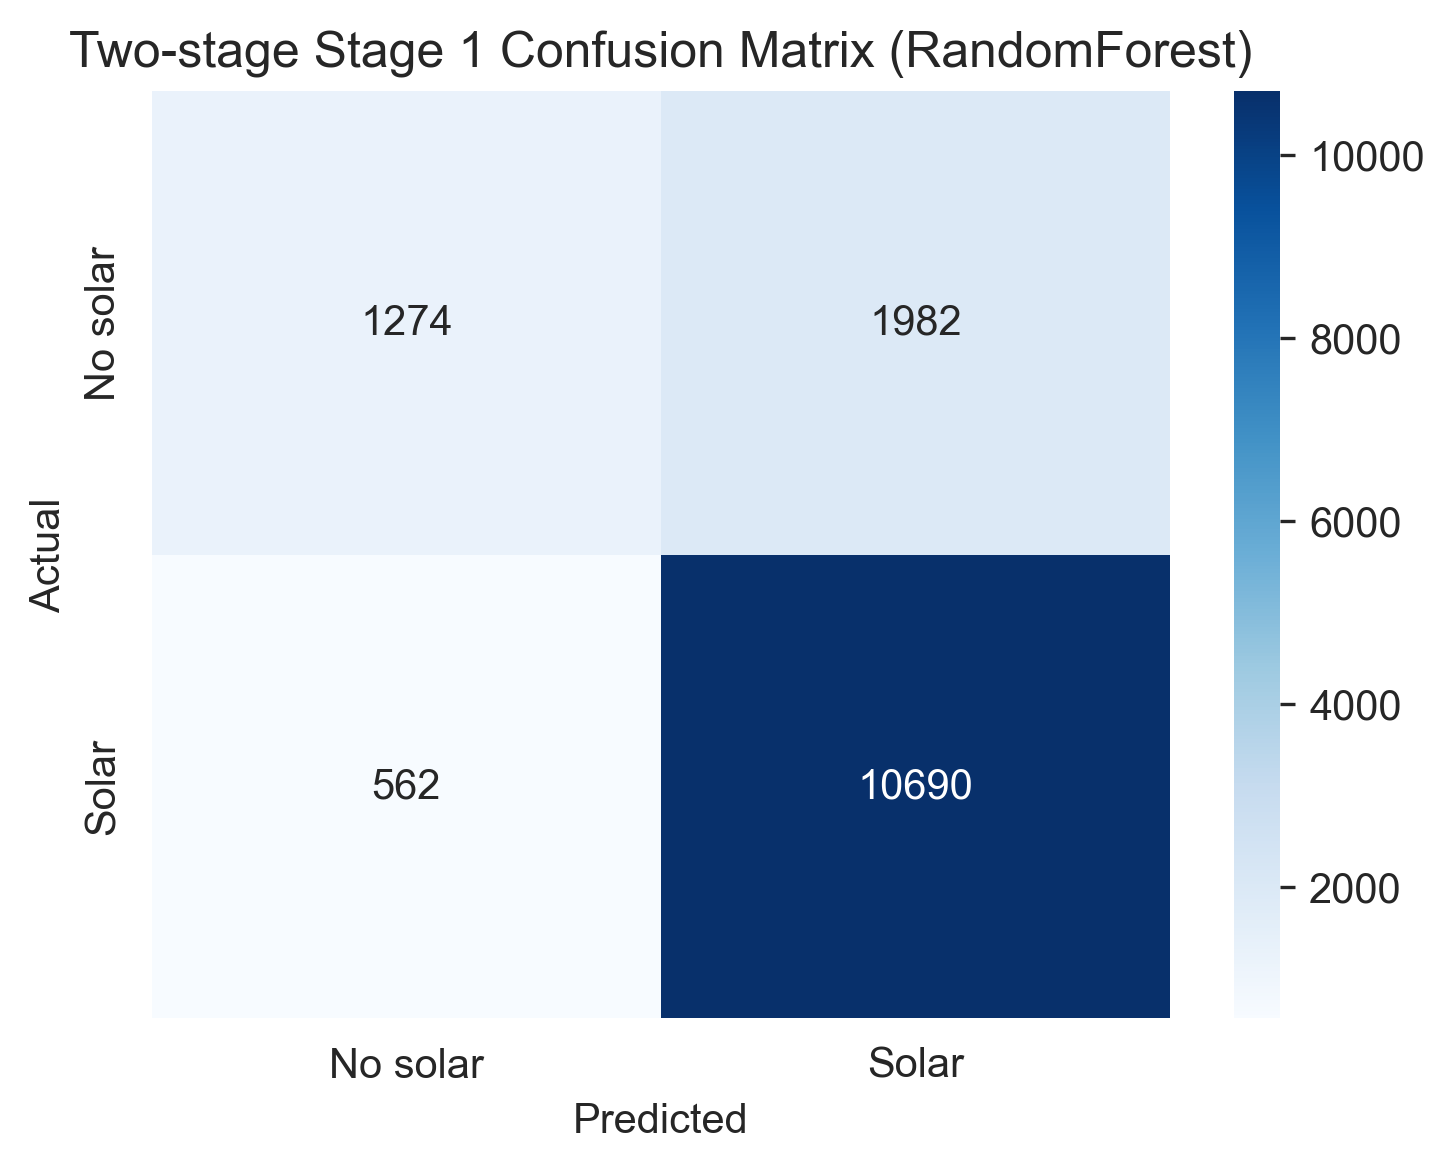
\includegraphics[width=\linewidth]{outputs/figures/transfer/03_twostage_stage1_confusion_matrix_voted.png}
\end{minipage}
\hfill
\begin{minipage}[b]{0.48\linewidth}
\centering
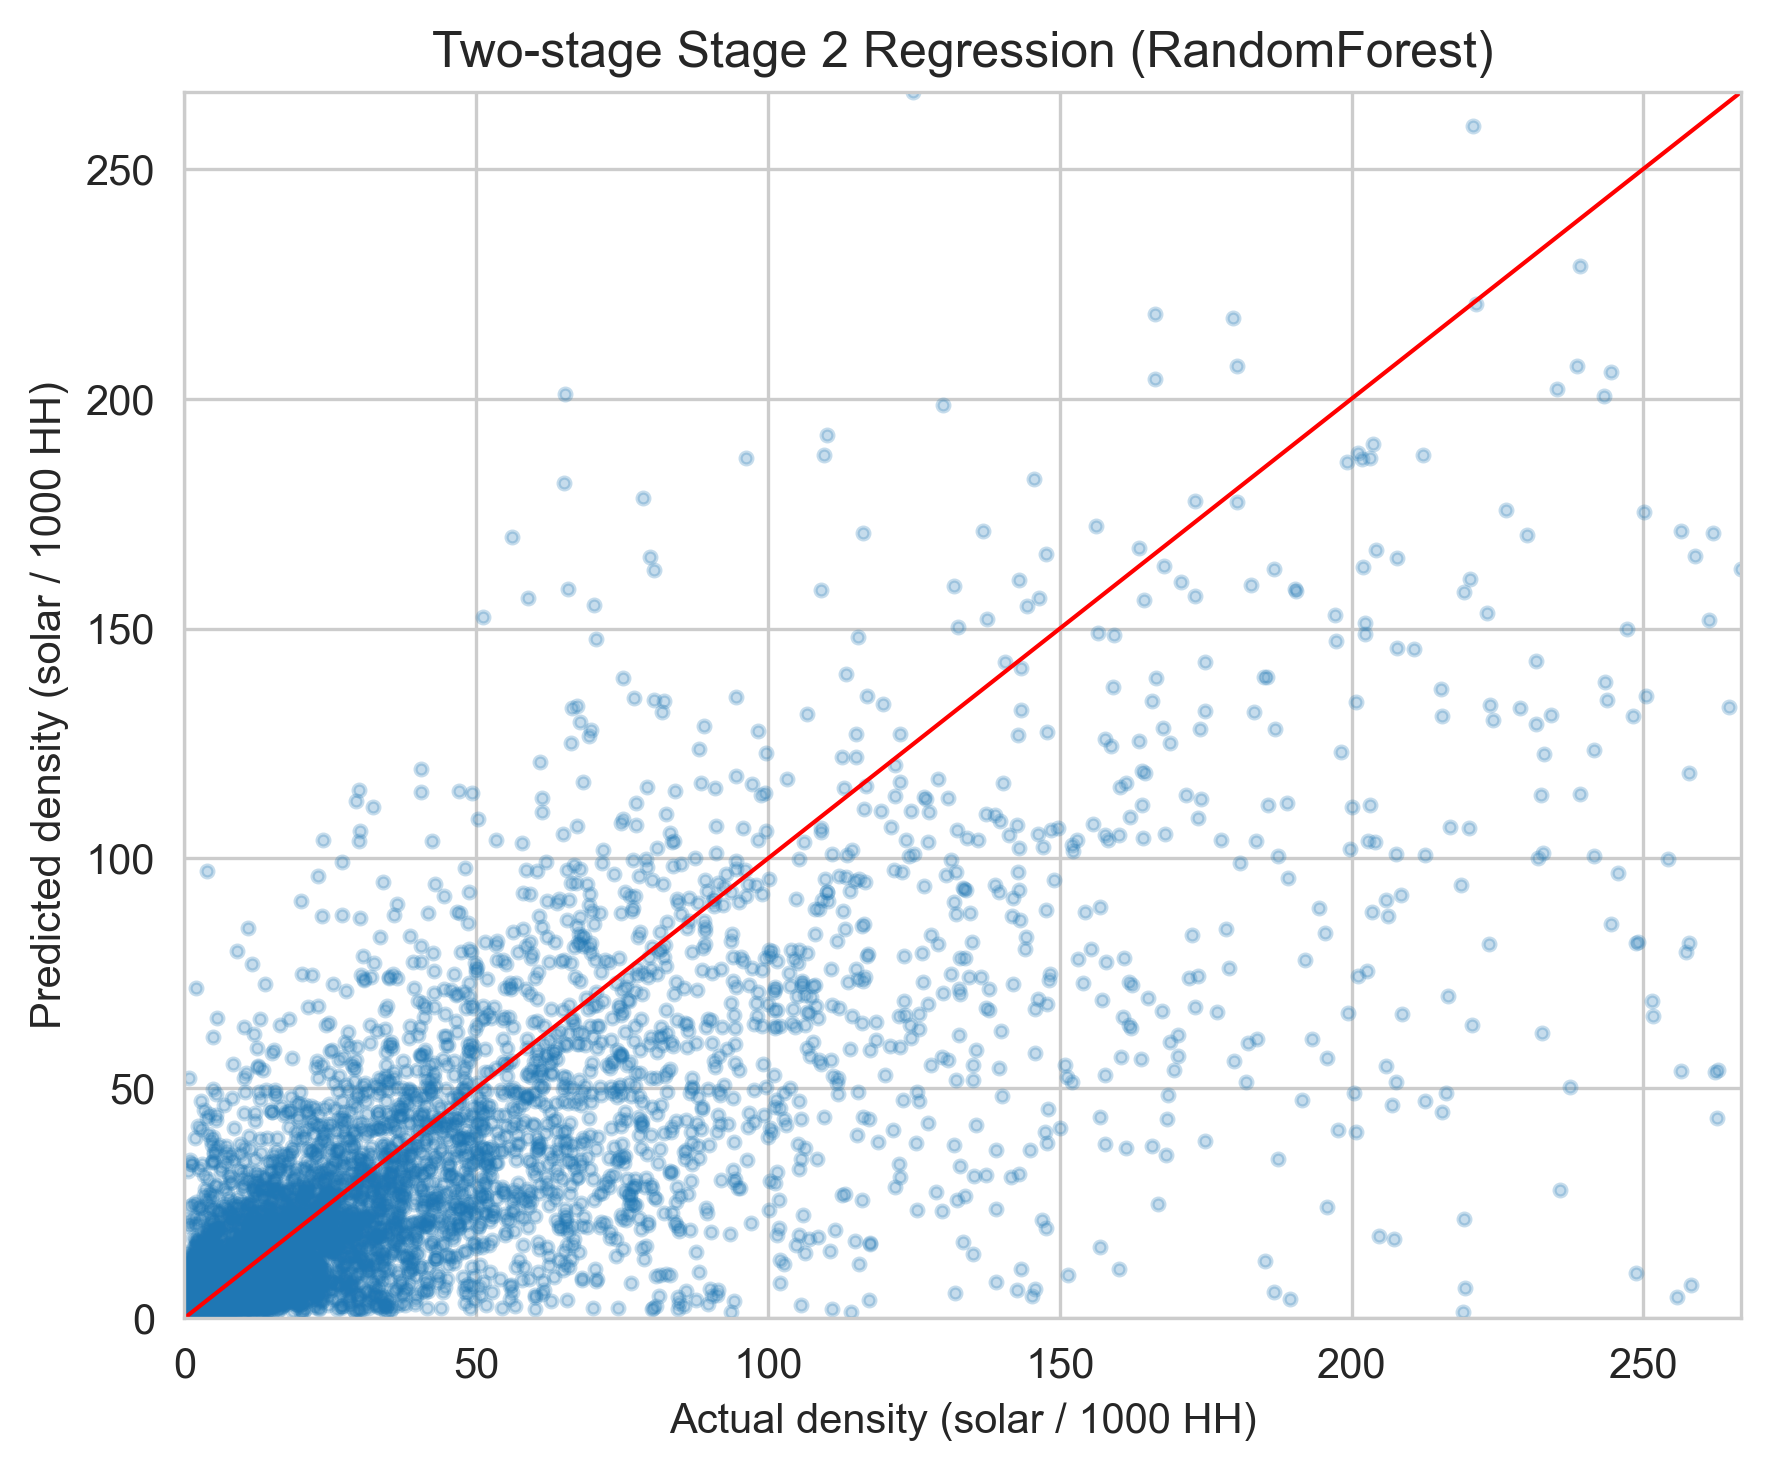
\includegraphics[width=\linewidth]{outputs/figures/transfer/03_twostage_stage2_predicted_vs_actual_voted.png}
\end{minipage}
\caption{Two-Stage 模型結果：（左）Stage~1 混淆矩陣；（右）Stage~2 預測對實際值（log1p 尺度）}
\label{fig:twostage_results}
\end{figure}

% =========================================================
\section{跨國遷移：臺灣推論}
% =========================================================

\subsection{特徵對應與資料整合}

本研究篩除美國特有欄位後，以 Voted 特徵集（90 欄）訓練之 Two-Stage 模型遷移至臺灣。
臺灣端整合五類資料來源：
（1）\textbf{氣候}：NASA POWER API 之年均日照輻射量、溫度、濕度、風速；
（2）\textbf{電力}：台電鄉鎮用電統計之住宅與商業用電量、電價；
（3）\textbf{人口}：內政部戶政司之年齡結構、人口密度、戶均規模；
（4）\textbf{收入}：主計總處家庭收支調查之家戶可支配所得中位數；
（5）\textbf{政策}：經濟部能源局各鄉鎮 FIT 躉購費率（含離島與東部加成）。

以 TOWNCODE（鄉鎮市區代碼）為鍵，合併為 368 列（全臺鄉鎮市區）之 master table。
90 個美國特徵中，28 個可直接對應，主要涵蓋氣候、電力、人口與收入；其餘 62 個缺口欄位以美國中位數插補。
換言之，本研究不假設臺灣能完整重建 DeepSolar，而是測試：在核心能源經濟訊號保留、非核心欄位以中性值補足的情況下，模型是否仍能提供有用排序。
此設計雖然保守，但也較符合實務場景：對多數國家或地方政府而言，短期內通常無法蒐集與美國普查區完全同構的住宅、教育、職業與通勤資料，因此方法若要具備移植價值，便需容忍一定程度的資料缺口。

\subsection{推論結果}

模型最終對臺灣 368 個鄉鎮市區輸出 Stage~1 部署機率、Stage~2 密度預測及綜合分數（combined score）。
Stage~1 部署機率大致集中在 0.75--0.88 之間，顯示模型對多數臺灣鄉鎮皆判定具有一定部署可能性；
Stage~2 密度預測則保留較明顯的區域差異，形成後續排序所需的辨識力。
圖 \ref{fig:taiwan_pred} 顯示三項輸出的整體分布，說明跨國遷移後的模型分數並未集中於極端區間，而是保有可排序的變異性。

\begin{figure}[H]
\centering
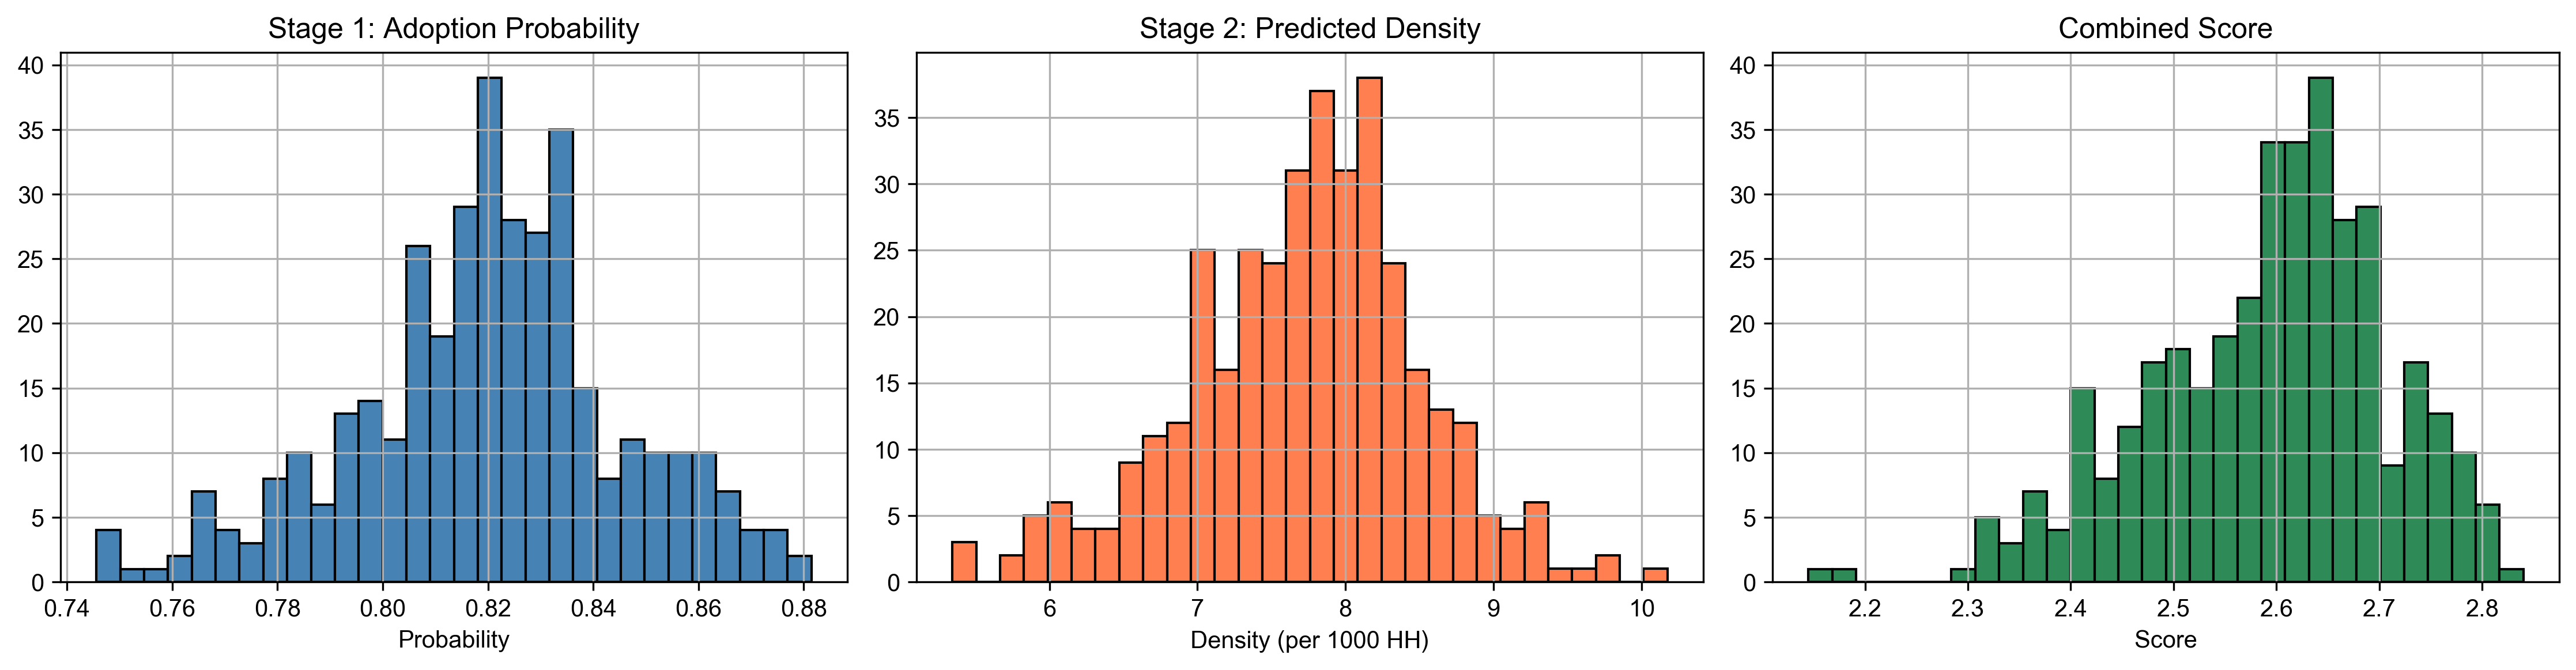
\includegraphics[width=0.82\linewidth]{outputs/figures/transfer/04_taiwan_prediction_distribution.png}
\caption{臺灣 368 鄉鎮市區推論結果分布：（左）Stage~1 部署機率；（中）Stage~2 預測密度；（右）綜合分數}
\label{fig:taiwan_pred}
\end{figure}

% =========================================================
\section{MADA 推廣優先序排序}
% =========================================================

\subsection{TOPSIS 方法與準則設計}

本研究採用 TOPSIS（Technique for Order Preference by Similarity to Ideal Solution）\citep{hwang1981topsis} 對 368 個鄉鎮市區進行排序。
實作上採 min-max 標準化，依權重加總後計算各方案與正、負理想解之距離，得到相對貼近度分數。

值得注意的是，本研究刻意將 \textbf{鄉鎮排序} 與 \textbf{縣市背景資訊} 分開：
前一版曾將 FIT、教育與就業等縣市層級變數直接放入鄉鎮 TOPSIS，造成整個縣市因共同加成而整批前移。
因此，本版只保留真正具有鄉鎮差異的訊號作為排序準則，並將 FIT、教育、就業與房價保留作背景解讀，而非直接參與第一層排序。

最終納入鄉鎮 TOPSIS 之四項準則與權重如表 \ref{tab:topsis_criteria}。

\begin{table}[H]
\caption{TOPSIS 準則與權重}
\label{tab:topsis_criteria}
\centering
\small
\begin{tabular}{lcp{5.5cm}}
\toprule
準則 & 權重 & 說明 \\
\midrule
combined\_score & 0.55 & 美國 Two-Stage 模型輸出之相對部署傾向 \\
daily\_solar\_radiation & 0.20 & 年均日照輻射量（kWh/m$^2$/day） \\
occupancy\_owner\_rate & 0.15 & 自有住宅率，作為屋頂決策可行性 proxy \\
log\_median\_household\_income & 0.10 & log（家戶可支配所得中位數），支付能力 proxy \\
\bottomrule
\end{tabular}
\end{table}

\subsection{排序結果}

排序結果以前述修正版更符合直覺。
前段主要集中於屏東、高雄與臺南平原地區，例如屏東縣九如鄉、萬丹鄉與臺南市關廟區，兼具高模型潛力、穩定日照與較高住宅自有率；
末段則多為山地或偏遠鄉鎮，如苗栗縣泰安鄉、新竹縣五峰鄉與臺中市和平區，反映低人口密度、地形限制與住宅條件不足的綜合作用。

表 \ref{tab:top_bottom} 列示優先序最高與最低之鄉鎮市區。
值得注意的是，前段名單不再由同一離島縣市整批占據，而是以南部平原區為主；這正是將縣級常數從鄉鎮 TOPSIS 中移除後的直接效果。

\begin{table}[H]
\caption{TOPSIS 優先序最高與最低之鄉鎮市區（各 6 名）}
\label{tab:top_bottom}
\centering
\small
\begin{tabular}{clcc|clcc}
\toprule
排序 & 縣市 & 鄉鎮 & 分數 & 排序 & 縣市 & 鄉鎮 & 分數 \\
\midrule
1 & 屏東縣 & 九如鄉 & 0.872 & 363 & 臺東縣 & 長濱鄉 & 0.315 \\
2 & 屏東縣 & 萬丹鄉 & 0.872 & 364 & 臺中市 & 中區 & 0.275 \\
3 & 臺南市 & 關廟區 & 0.856 & 365 & 花蓮縣 & 豐濱鄉 & 0.267 \\
4 & 高雄市 & 仁武區 & 0.855 & 366 & 臺中市 & 和平區 & 0.258 \\
5 & 高雄市 & 大寮區 & 0.854 & 367 & 新竹縣 & 五峰鄉 & 0.143 \\
6 & 屏東縣 & 里港鄉 & 0.854 & 368 & 苗栗縣 & 泰安鄉 & 0.130 \\
\bottomrule
\end{tabular}
\end{table}

圖 \ref{fig:taiwan_map} 以鄉鎮熱力圖呈現最終排序結果，可見高潛力區主要落在南部平原帶，離島雖仍具一定潛力，但已不再因縣級加成而集體位居最前段。

\begin{figure}[H]
\centering
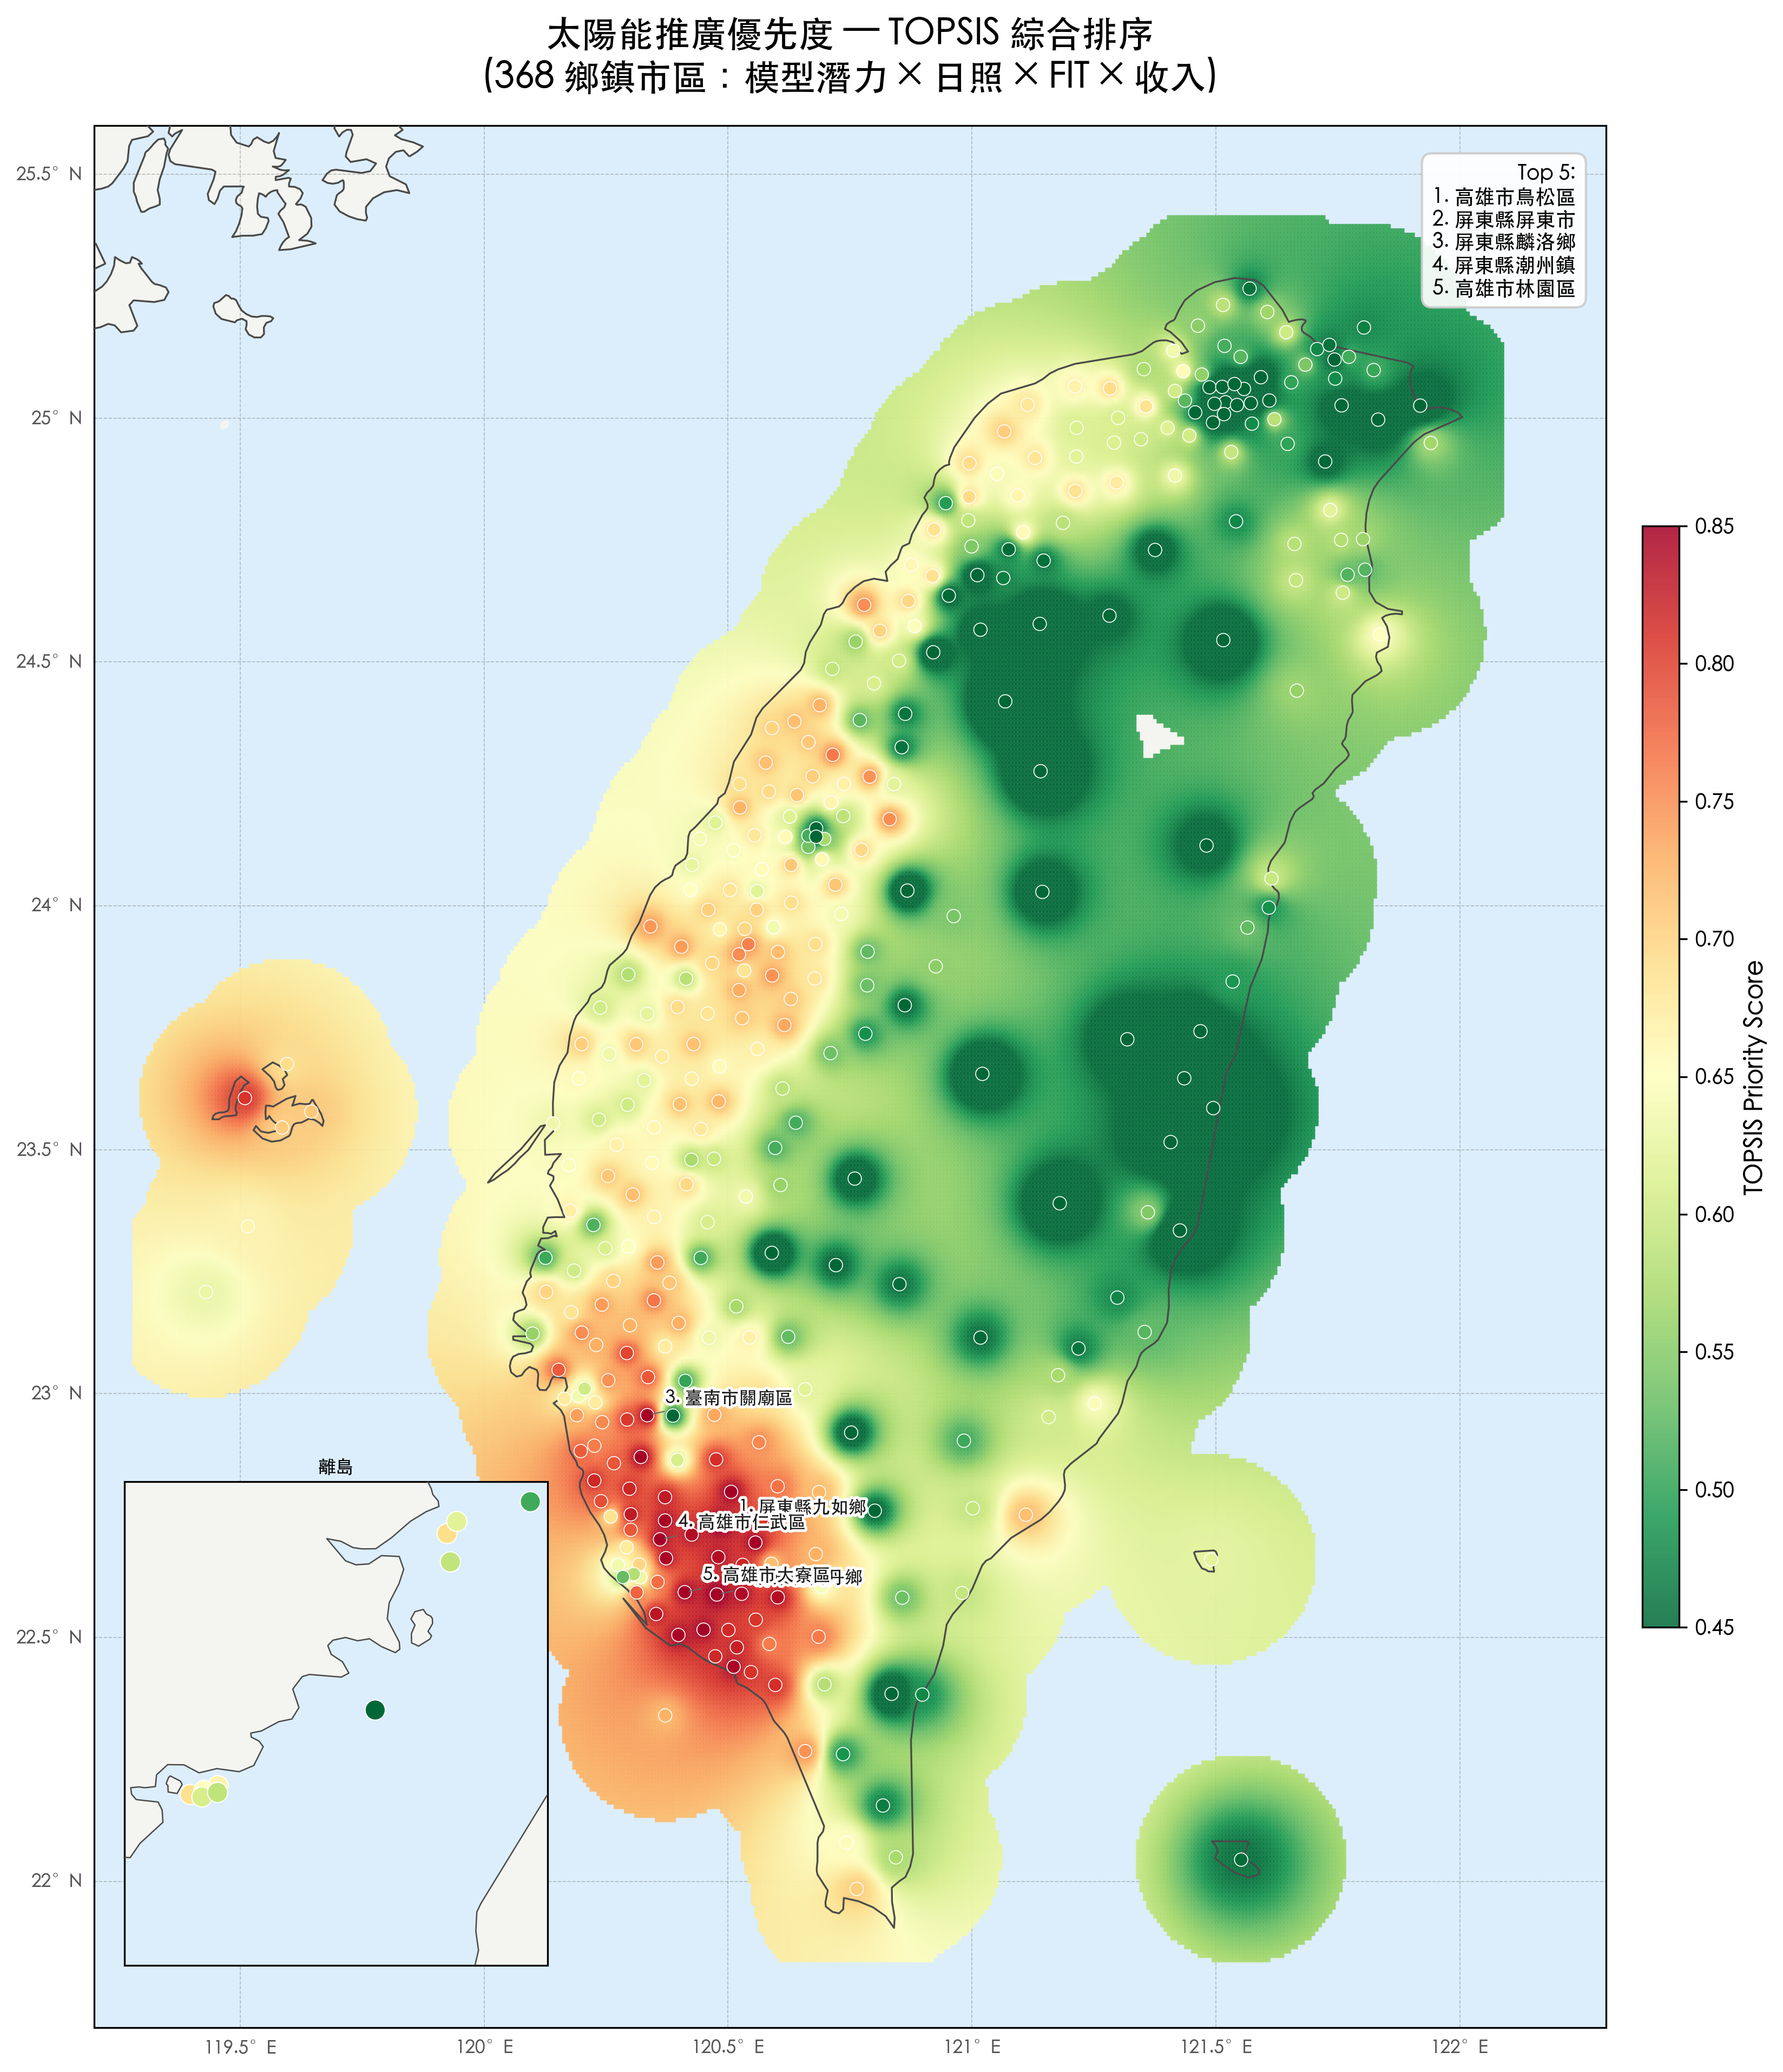
\includegraphics[width=0.85\linewidth]{outputs/figures/transfer/map_01_topsis_heatmap.png}
\caption{臺灣鄉鎮市區太陽能推廣優先度熱力圖（TOPSIS 綜合分數）}
\label{fig:taiwan_map}
\end{figure}

從區域分布來看，此結果亦與臺灣既有光電發展經驗大致一致。
南部平原地區具備較高日照、較完整平地聚落與相對成熟之農業及工業用地配置，因此在模型與排序中同時表現突出；
反之，山地鄉與偏遠地區即使局部日照條件不差，仍可能因建築密度、可利用屋頂與電網條件受限而落於後段。
這也說明排序結果應理解為「綜合部署潛力」，而非僅由單一自然條件所決定。

% =========================================================
\section{外部驗證}
% =========================================================

本研究以經濟部能源局「歷年各縣市太陽光電裝置容量」為 ground truth，取 114 年（2025）最新完整年度資料進行外部驗證。
考量縣市總容量會受到行政區規模影響，本研究不再以「縣市平均分數對縣市總容量」作單一檢驗，而是拆成兩種尺度：
（1）\textbf{平均鄉鎮潛力}（\texttt{mean\_topsis}）對 \textbf{每鄉鎮平均裝設量}（\texttt{capacity\_per\_town\_kw}）；
（2）\textbf{縣市總分}（\texttt{sum\_topsis}）對 \textbf{縣市總裝設量}。

驗證結果如圖 \ref{fig:validation} 所示。
若以縣市平均鄉鎮分數對每鄉鎮平均裝設量衡量，Spearman $\rho = 0.600$（$p = 0.003$）；
若以縣市總分對縣市總裝設量衡量，則達 $\rho = 0.878$（$p<0.001$）。
此外，原始模型綜合分數（\texttt{mean\_combined}）對每鄉鎮平均裝設量之相關為 $\rho = 0.441$（$p = 0.040$），顯示經過修正後的 TOPSIS 排序，相較單純依賴模型分數，更能貼近臺灣實際部署分布。

這代表兩件事：
第一，美國基準模型保留了可遷移的核心訊號；
第二，當 MADA 僅納入具鄉鎮差異的準則時，排序結果的實務解釋力會明顯提升。
若從解釋角度觀察，縣市總分與總裝設量的高度一致，反映本模型對「整體部署規模」的掌握較佳；
而平均鄉鎮分數與每鄉鎮平均裝設量的顯著正相關，則表示此排序在比較縣市內部平均推廣潛力時亦具有參考價值。

\subsection{限制與討論}

儘管驗證結果支持本研究方法之可用性，仍須注意三項限制。
第一，臺灣端可直接對應之特徵僅 28 項，仍有相當比例仰賴插補，因此目前排序更適合作為前期篩選工具，而非最終投資決策依據。
第二，外部驗證使用之指標為縣市層級實際裝設量，無法完全反映鄉鎮內部差異，故相關係數應解讀為整體趨勢一致性，而非逐點預測精度。
第三，現行模型尚未納入電網饋線容量、屋頂可利用面積、工業區土地條件等物理限制，這些因素對實際案場落地具有關鍵影響。
因此，本研究所產出的排序較接近「優先調查名單」，仍需與工程、土地及政策可行性評估結合，方能形成完整決策。

\begin{figure}[H]
\centering
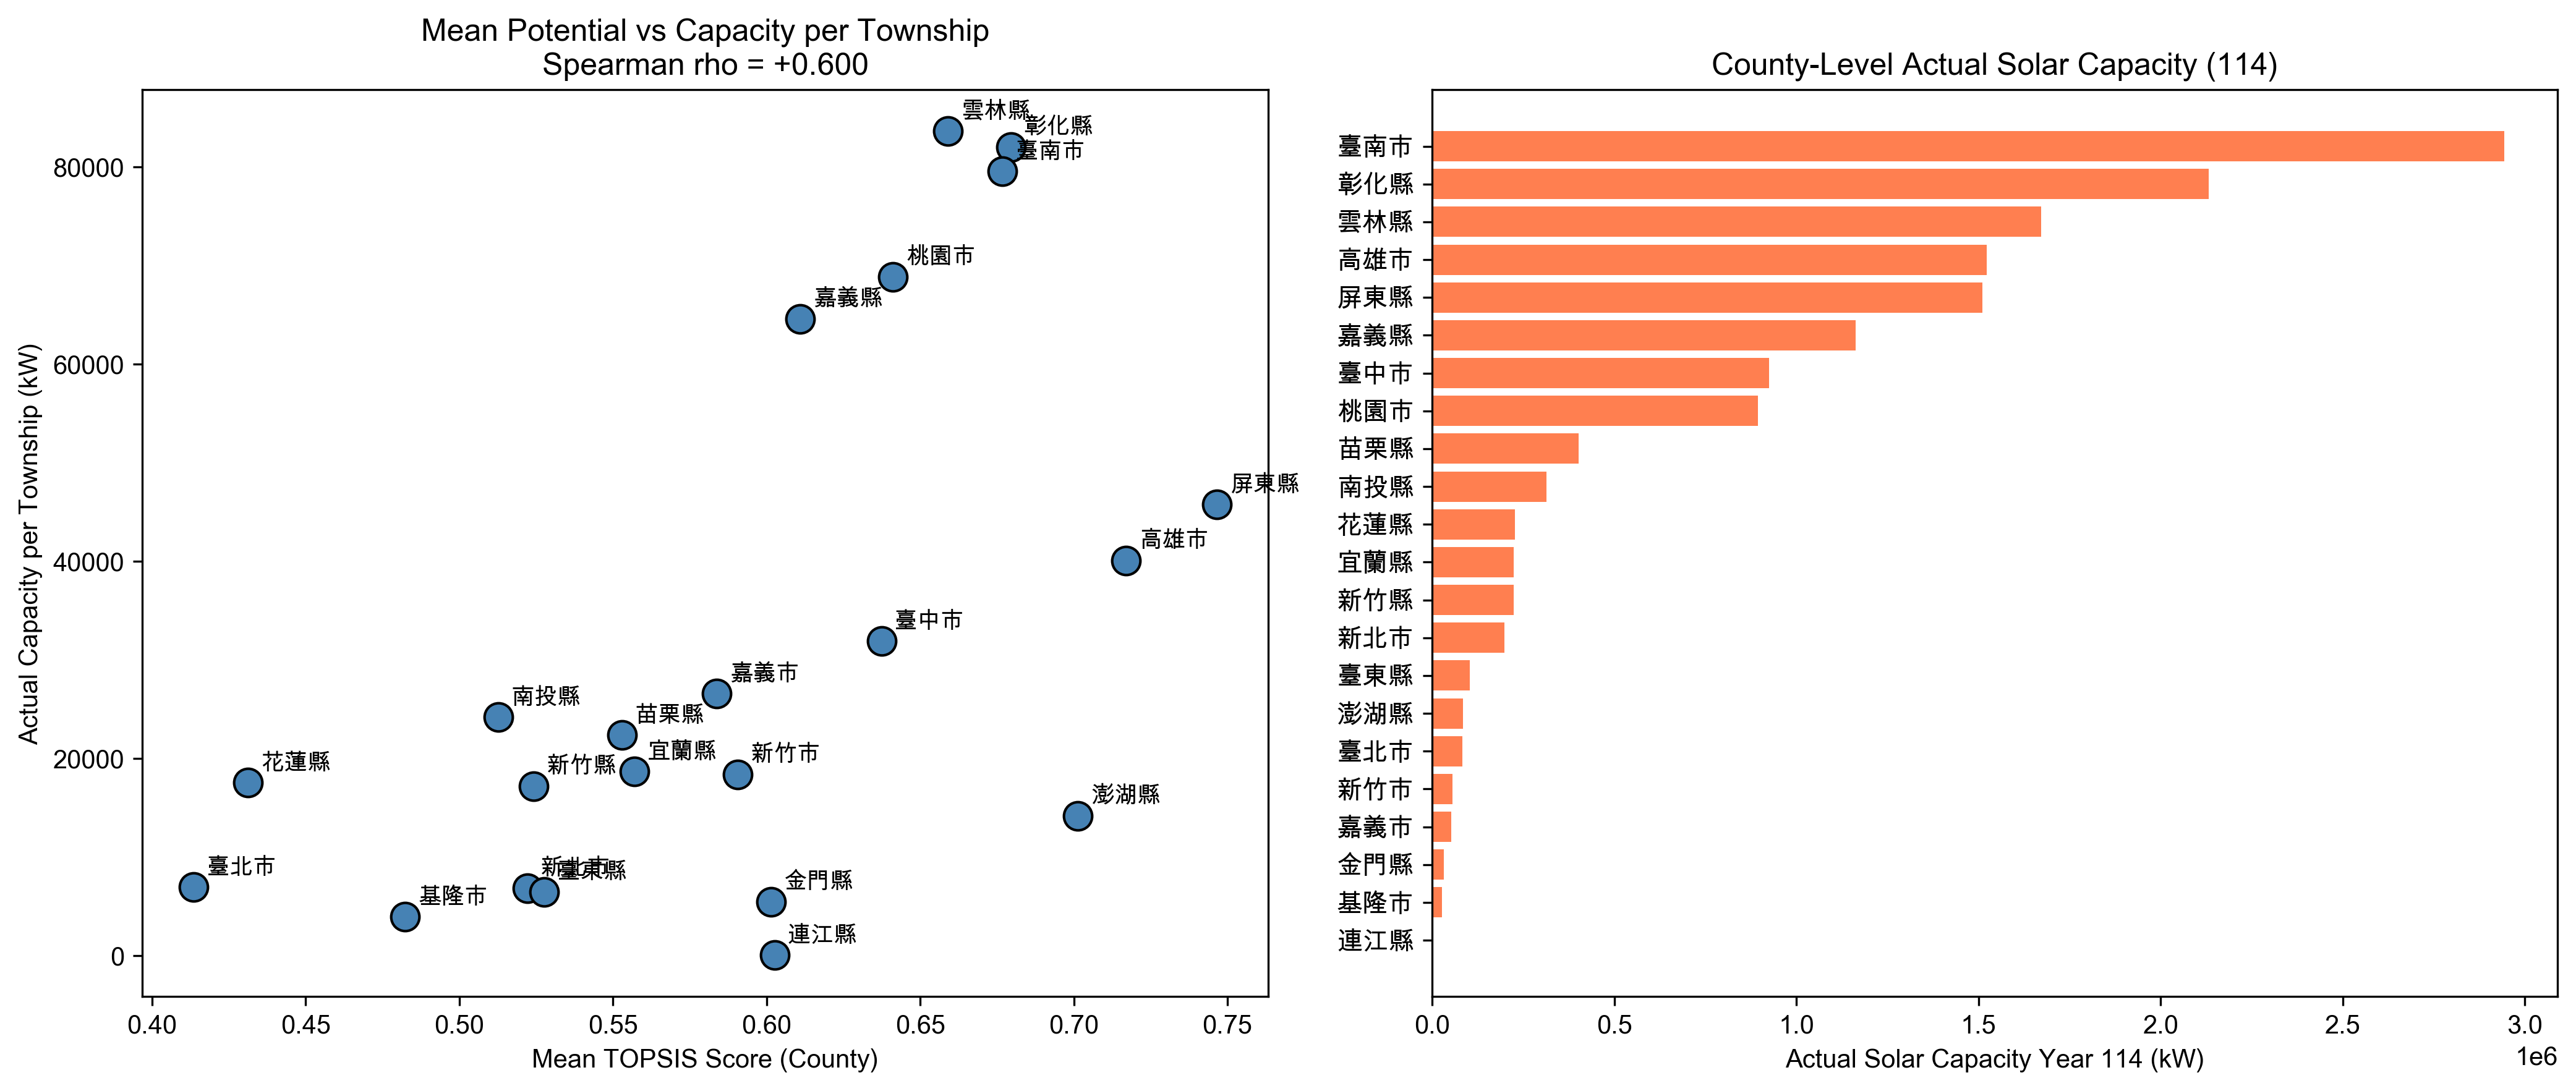
\includegraphics[width=0.9\linewidth]{outputs/figures/transfer/06_external_validation.png}
\caption{外部驗證：縣市平均鄉鎮 TOPSIS 分數對每鄉鎮平均裝設量（左），以及 114 年縣市實際太陽光電裝置容量（右）}
\label{fig:validation}
\end{figure}

% =========================================================
\section{結論}
% =========================================================

本研究完成一套從美國 DeepSolar 到臺灣鄉鎮排序的跨國遷移流程。
其核心貢獻不只在於訓練出一個預測模型，而是提出一條可操作的故事線：
先辨識哪些特徵可以跨國保留，再以 Two-Stage 模型建立穩定基準，最後將模型輸出轉換為臺灣地方決策可理解的推廣順序。

研究結果顯示，Two-Stage 模型在美國端具穩定表現，而修正後的 MADA 設計在臺灣端也與實際裝設量呈顯著正相關。
這說明跨國遷移不必追求完全重建原始資料結構，只要保留核心訊號並審慎處理決策準則，仍可得到具實務價值的區域排序結果。

未來可進一步納入真正的鄉鎮級物理限制資料，例如屋頂可用面積、建物型態與饋線容量，以提升排序結果對真實案場可行性的貼近程度。

% =========================================================
% \section*{參考文獻}
% Remove "References" section title from the table of contents
\begin{thebibliography}{99}

\bibitem[Yu et al.(2018)]{dubey2021deepsolar}
Yu, J., Z. Wang, A. Majumdar, and R. Rajagopal (2018), ``DeepSolar: A Machine Learning Framework to Efficiently Construct a Solar Deployment Database in the United States,'' \textit{Joule}, 2(12), 2605--2617.

\bibitem[Hwang and Yoon(1981)]{hwang1981topsis}
Hwang, C.L. and K. Yoon (1981), \textit{Multiple Attribute Decision Making: Methods and Applications}, Springer-Verlag, Berlin.

\end{thebibliography}

\end{document}
